\chapter{A Conceptual Framework for Information Discovery and Curation on the Web}
\label{chapter:framework}

Although Web-based information discovery and curation tasks are commonly performed, there is a lack of literature on how to enable and support them when building Web applications. I reduce this gap by presenting a framework of design factors to facilitate digital information discovery and curation. In my framework, I build on existing models and frameworks of information discovery and curation and my analysis of existing Web tools to derive corresponding design factors for Web design. The first part of the framework deals with the \textit{motives} behind information discovery and curation (see Section~\ref{section:motives}). These motives often define use cases for Web application design and help set initial assumptions about required functionality.

The second part of the framework defines the \textit{actions} that comprise discovery and curation activities, and the design factors that enable those actions (see Section~\ref{section:enablers}). Some examples of actions include managing and preserving information. In order to enable these actions, a Web-based application must provide corresponding mechanisms, such as bookmarking and tagging capabilities.

\pagebreak
Actions can be further decomposed into \textit{operations} performed using mechanisms that enable the actions. For example, information preservation (action) can be enabled using a bookmaking feature (enabling mechanism) so that users can bookmark information using the feature (operation). Therefore, the remaining part of the framework deals with improving operations that are involved in information discovery and curation (see Section~\ref{section:enhancing}).  

On the whole, in my framework I consider human motives and relate information discovery and curation actions with corresponding enabling mechanisms. Similarly, I relate operations, that arise from actions, with corresponding cognitive support, personalization, and automation.  Similar terminology is used in Activity Theory~\cite{kuutti1996activity} to describe human practices. 

Figure~\ref{fig:framework_overview} gives a high-level overview of the framework and illustrates how the different components of the framework are connected.



\begin{figure}[ht!]
	\noindent
	\centering
    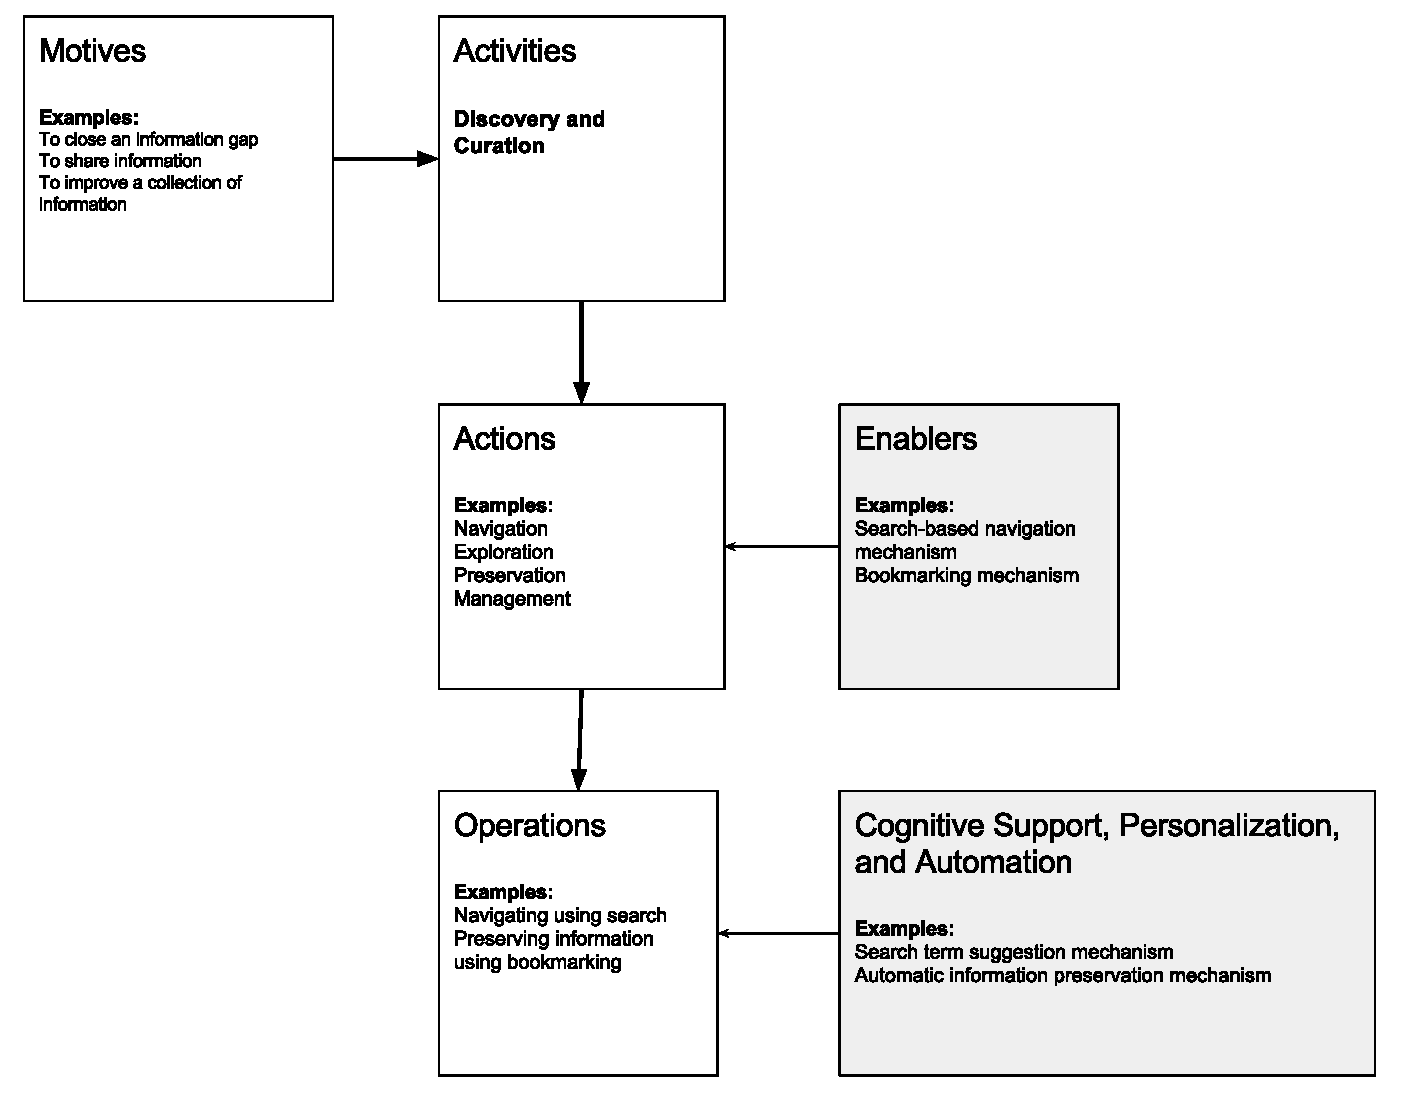
\includegraphics[width=\linewidth]{framework_overview.pdf}
	\caption{Framework Composition}
	\label{fig:framework_overview} 
\end{figure}
\clearpage

{\section{Motives Behind Information Discovery and Curation}

\label{section:motives}
\begin{figure}[ht!]
	\noindent
	\centering
    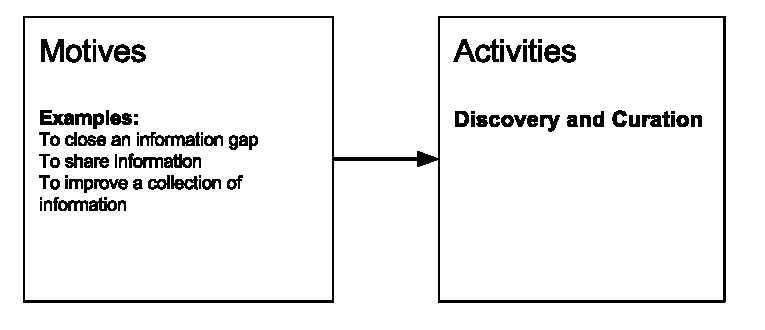
\includegraphics[width=\linewidth]{motives.pdf}
	\caption{Section Overview: Motives Behind Information Discovery and Curation}
	\label{fig:motives} 
\end{figure}

There are a wide variety of user motives behind information discovery and curation, and certain aspects of these motives can significantly impact the design of an application. Understanding a user's motives can help form a conceptual model of a needed Web application and its features. The following generalizations of motives and their properties can help define conceptual models and identify primary information discovery and curation use cases. Figure~\ref{fig:motives} illustrates the part of the framework discussed in this section.  

{\subsection{Closing a Knowledge Gap}
The primary motive for information discovery is usually to close a knowledge gap that occurs when the user tries to accomplish a task and lacks information to do so. This motive can take up various forms, which often depends on the nature of the information need and other conditions surrounding the given motive.        

Depending on the context in which it arose, an information need can have various degrees of specificity. For example, if the motive is to find inspiration for a project, the information need is vaguely defined. However, if the motive is to find a phone number of a specific business, an information need is well-defined. In some cases, the information need may be hidden and the user might not be aware of the existing knowledge gap. The specificity of an information need determines important properties of information discovery mechanisms, such as whether users can benefit more from mechanisms that allow them to specify an information need, help form an information need, or allow them to randomly retrieve information. This property has to be taken into consideration when evaluating or designing a Web application. 

The nature of an information need predetermines whether discovery is respectively serendipitous or oriented towards fact finding. Therefore, depending on the user needs, an application can be designed to increase serendipity and opportunistic discovery or to improve purposeful fact finding. On the one hand, displaying featured content can improve serendipitous discovery because of its unexpected nature and novelty. On the other hand, using context (e.g., location and date) to tailor search results to the user can improve fact finding. 

Another type of motive for information discovery relates to the two qualities of the Web defined by Lindley et al. -- temporality and persistence~\cite{lindley2012s}. \textit{Persistence} refers to the quality of the Web that allows people to habitually revisit Web pages and continue on-going Web projects. \textit{Temporality} refers to the quality of the Web that allows the content of Websites to be continuously updated to provide users with new information. Persistence alone usually facilitates information \textit{rediscovery}, which is an act of refinding previously found information. However, if persisitence is combined with temporality, they can facilitate discovery of new information within the same application or channel. I refer to this type of discovery as \textit{channel-based discovery}. Some of the common motives for channel-based discovery include orienting (or monitoring for updates) and opportunistic information discovery~\cite{lindley2012s}.          

The motive behind information rediscovery involves finding previously discovered information and reclosing the previously closed knowledge gap (e.g., in case the information was forgotten). It usually results in the user looking for previously found resources and Web pages. In fact, Web page revisitation is one of the most commonly performed Web browsing activities~\cite{adar2008large,cockburn2003improving}. The percentage of revisited web pages involved in Web browsing can range from 58\%~\cite{tauscher1997people} to 81\%~\cite{cockburn2001web}. Some of the reasons for revisiting pages include shopping, communication, entertainment, education, activity planning, and hobby-related information retrieval~\cite{adar2008large} (e.g., travel, fitness, and cooking). Some Web pages and resources can be rediscovered using navigation while others need to be previously preserved (bookmarked) in order to allow rediscovery. Rediscovery is one of the many ways in which information discovery and curation interweave. 
}

{\subsection{Supporting Future Use and Reaccess}
The main motive behind information curation is to make it possible to retrieve and use information. In order to facilitate easy information retrieval, many Web applications employ various forms of bookmarking systems. Traditionally, bookmarks must be manually organized into folders. However, this method of organization has been found inefficient because folders with bookmarks become easily cluttered~\cite{abrams1998information}. Therefore, in order to efficiently support information rediscovery, Web tools need to provide mechanisms for information preservation along with information management.
}

{\subsection{Improving Collections}
Reportedly, people gather information to improve existing collections~\cite{lindley2012s}. Although some deeper motives may include self reflection or the possibility of future use, collecting information is a motive in itself. In general, information gathering may be stretched over a period of time~\cite{kellar2006goal}, resulting in repeated page visitation. Although information gathering comprises only 13.4\% of Web usage, it highly contributes to various goal-supporting activities, such as decision making and planning~\cite{kellar2006goal}.

}

{\subsection{Facilitating Communication}
As part of his information behavior model, Wilson identified communication of information as an outcome of information seeking. Communication can also be thought of as a motive for information discovery and curation. To support communication of information, Web tools have to provide mechanisms that allow various users to share information among themselves. 

\textit{Social bookmarking} is a way to preserve and share information within various communities. In recent years, it has gained popularity as an effective way of communicating with other users~\cite{estelles2010social}. One of the first visions of social bookmarking was associated with Web blogging. Oravec~\cite{oravec2002bookmarking} believes that web blogs help users annotate or bookmark important information and build a ``map'' of the Internet. The evolution of social bookmarking has led to advanced bookmarking technologies and provided a means for collaborative information discovery and curation. 
}
{\subsection{Summary}
While it is not feasible to list all of the possible motives for information discovery and curation, in this section I outline some of the key motives that can aid in developing use cases and formalizing conceptual models for Web applications. These motives also make it easier to showcase how mechanisms for discovery and curation (presented in the next section) complement each other.
} 
}

{\section{Discovery and Curation Activities, Actions, and Their Enablers}
\label{section:enablers}

\begin{figure}[ht!]
	\noindent
	\centering
    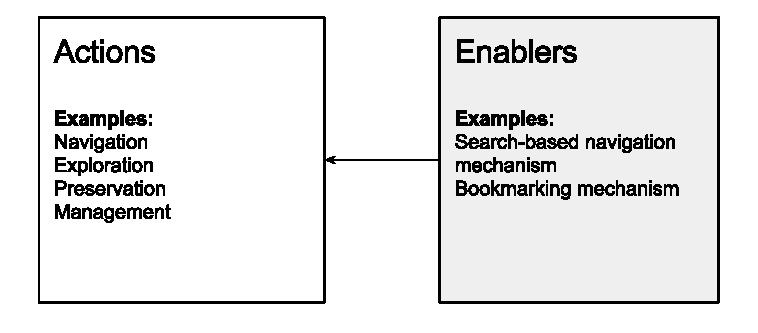
\includegraphics[width=\linewidth]{enablers.pdf}
	\caption{Section Overview: Discovery and Curation Activities, Actions, and Their Enablers}
	\label{fig:enablers_overview} 
\end{figure}
The next part of the framework (see Figure~\ref{fig:enablers_overview}) deals with the actions associated with enablers of information discovery and curation. A more detailed overview is depicted in Figure~\ref{fig:enablers}; the two main activities (discovery and curation) are decomposed into actions, and each of the actions is supported by a group of features or mechanisms that enable a given aspect of discovery or curation in a Web application. Examples of these enabling mechanisms can be found in Appendix~\ref{chapter:appendix_features}. The following subsections describe each of the feature groups and outline the corresponding questions a designer could ask to improve application design and evaluation.  

{\subsection{Navigation in Discovery: Following Information Scent}
In order to discover information, a user needs to have a way of navigating to it. Navigation in information discovery can be thought of as following an information scent. In general, information scent models deal with how users identify value, cost, or the access path of information sources based on proximal cues, such as links, icons, categories, etc.~\cite{pirolli1999information}. Common methods of navigation that facilitate information discovery include descriptional, referential, opportunistic, and system-regulated (see Table~\ref{table:navigation}). 

{\subsubsection{Descriptional Navigation}
A navigation is descriptional when the user has a means of describing their information need. It is often implemented as \textit{search-based navigation} since it allows users to enter a search query and describe what they want to find. Some of the modern descriptional navigation systems are voice-activated. 

Almost every present-day Web application has implemented a search feature, with rare exceptions of applications that utilize other methods of navigation, such as StumbleUpon and certain shopping websites. Some Web applications are \textit{integrated} with others, enabling users to search multiple websites at once.    

There are numerous ways in which descriptional navigation supports information discovery. Search-based navigation often serves as an entry point for information seeking~\cite{levene2011introduction}. When the motive behind information discovery has a well-articulated information need, then the user can express their information need by entering a search query. 

Descriptional navigation can also help to rediscover information. However, it is not always a reliable way of refinding information ~\cite{cockburn2003improving}. In information portals that provide access to fairly ambiguous information and that have regularly updated information flow, the search feature is usually designed around retrieving information related to some general topic. In order to make search-based navigation a reliable way to rediscover information, it must return consistent results. 
} % end subsection

\pagebreak

\begin{figure}[ht!]
	\noindent
	\centering
    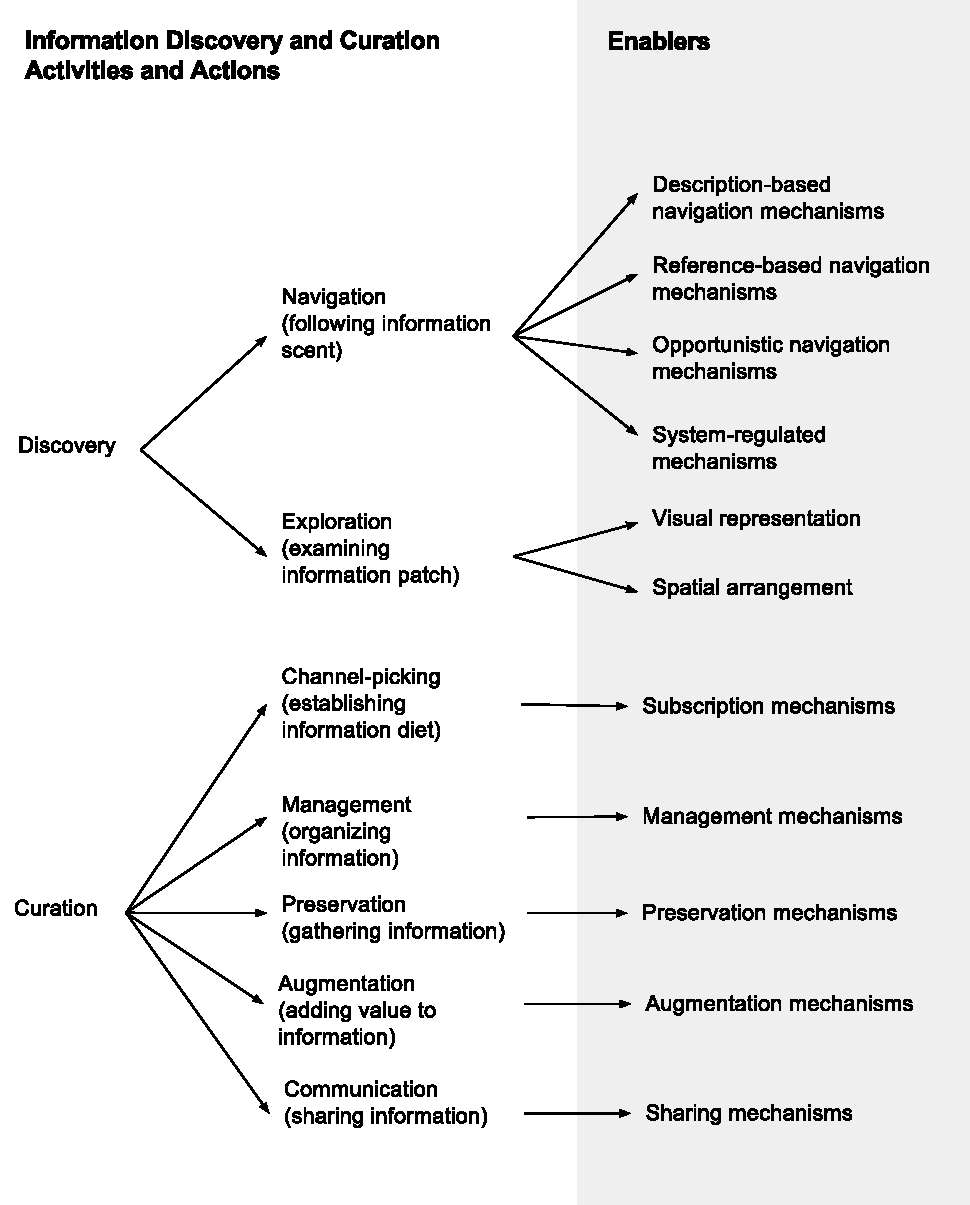
\includegraphics[width=\linewidth]{framework_enablers.pdf}
	\caption{Information Discovery and Curation Activities, Actions, and Corresponding Enablers}
	\label{fig:enablers} 
\end{figure}


{\subsubsection{Referential Navigation}
A navigation is referential when the user finds a reference to the term that they are looking for, such as a link or icon. This reference represents an information scent. The underlying assumption of this method of navigation is that the user can recognize the needed information or a reference to it as they see it~\cite{waterworth1991model}. 

Referential navigation mechanisms can take many forms. Some common types are \textbf{categories}, \textbf{facets}, \textbf{filters} and \textbf{tags}. In some applications, users can search by a given \textbf{resource}. For example, YouTube provides a playlist with music related to the currently playing song. Information scent representatives may also reference sources outside of the given system. This enables another type of \textbf{integration} of Web applications. 

Referential navigation can help the user identify their information needs by suggesting terms, topics or categories to use, and therefore, direct the user to relevant resources~\cite{levene2011introduction}. It can also help narrow the results to a specific type of resource so that further discovery is bounded by that type. For example, TripAdvisor helps narrow search resilts by allowing users to choose among hotels, flights, vacation rentals, restaurants and destinations.

} % end subsection


\begin{table}[ht!]
\caption{Navigation Mechanisms}
\label{table:navigation} 
\begin{tabular}{{| >{\raggedright}p{0.33\linewidth}|p{0.67\linewidth}|}}
\hline
Navigation mechanisms     	& Questions to be posed during the design or evaluation of  discovery and curation tools \\
\hline
&\\
\textbf{Descriptional} 			& \\
Search-based navigation							& Is it possible to navigate within the application using a search mechanism? \\
Integrated search				& Is it possible to retrieve information from  other applications using a search mechanism? \\
\textbf{Referential}       		& \\
Categories				 		& Is it possible to navigate using categories? \\
Facets				    		& Is it possible to navigate using facets? \\
Filters					  		& Is it possible to navigate using filters? \\
Tags				      		& Is it possible to navigate using tags? \\
Search by item or resource		& Is it possible to search by item or resource? \\
Integrated reference			& Is it possible to retrieve information from other applications using any of the referential mechanisms?\\
\textbf{Opportunistic}          & \\
Opportunistic navigation        & Is it possible to opportunistically navigate through information within the application? \\
Integrated opportunistic navigation        & Is it possible to opportunistically retrieve information from other applications? \\
&\\
\textbf{System-regulated}            		& \\
Static direct display           & Is it possible to view static information directly without active search? \\
Integrated static display   	& Is it possible to view static information from other applications without active search? \\
Featured content             	& Is it possible to view featured content? \\
Integrated featured content     & Is it possible to view featured content from other applications? \\
News feed             			& Is it possible to view news feeds? \\
Integrated news feed            & Is it possible to view news feeds from other applications? \\
&\\
\hline
\end{tabular}
\end{table}

{\subsubsection{Opportunistic Navigation}
Opportunistic navigation is a method of navigating `randomly' through resources and Web pages. I apply the term `opportunistic' to describe this type of navigation because it is not truly random, however, its serendipitous nature often makes users feel like it is. This navigation method is especially useful when the information need is fully undefined.

Many applications support \textbf{opportunistic navigation} to allow for opportunistic jumping from one resource to another. For example, StumbleUpon makes it possible to explore the Web in general --- other websites and Web applications, allowing for \textbf{integrated} navigation --- whereas Wikipedia provides opportunistic access to its own articles. 
} % end subsection

\pagebreak

{\subsubsection{System-regulated Navigation}
Web applications often display or update information without the user's active participation. This information can be a \textbf{news feed}, \textbf{featured} deals or articles, \textbf{static information}, or other types of content. In my thesis, I refer to this type of navigation as system-regulated because it occurs when the application brings the content to the user instead of the user applying any effort to find content. It differs from opportunistic navigation because the the user cannot choose when to observe new information; instead, all updates are regulated by the application. 

One example of an application that utilizes system-regulated navigation is Yelp. As soon as the user enters the site, this tool displays featured restaurants as well as the user's recent activities. As with any other navigation method, system-regulated navigation can ensure cross-application \textbf{integration} by displaying content from other Web applications. 
} % end subsection
} % end section

{\subsection{Exploration in Discovery: Examining Information Patches}
Exploration of resources is another action that facilitates information discovery. Visual and spatial cues, which help representing single or multiple resources, enable this action by allowing users to conveniently examine information patches (see Table~\ref{table:exploration}). 


Abrams et al.~\cite{abrams1998information} identified link representation as one of the problems with traditional bookmarking. Analogous with browsing through a bookmark manager, identifying relevant information when browsing through links in a Web application can be a challenging task. \textbf{Visual} and \textbf{textual previews} make it easier to evaluate the relevance of resources by providing the user with more information scent. Many social bookmarking systems, such as Scoop.it! and Pinterest, support visual previews of bookmarked pages. Delicious is a social bookmarking application that lacks this type of link representation support, and therefore, it is harder to determine if a link will lead to a relevant resource.

\textbf{Visual} and \textbf{textual} information cues and representations are also important for a single resource exploration. Not only do they help navigating within the resource or Web page, but they can also contribute to the learning experience. For example, if the user would like to know what something looks like, they can learn it from the representation in question.  

Similar to link representation, spatial visualization of numerous links is another problem that occurs when browsing through diverse content~\cite{abrams1998information}. Therefore, a semantic to the \textbf{spatial arrangement} of information (single and multiple resources) is of major importance. Information discovery applications often employ sophisticated ways of spatially arranging resources to make it easier to browse through large amounts of information. For example, many tools use a `pinboard' layout of resources similar to Pinterest. Common ways of arranging multiple resources include list, grid, and gallery layouts. Additionally, \textbf{consistency} in the way multiple and single resources are represented helps form a conceptual model of how the application can be used and provides some degree of predictability~\cite{norman2002design}.

\begin{table}[ht!]
\caption{Visual and Spatial Exploration Mechanisms}
\label{table:exploration} 
\begin{tabular}{{| >{\raggedright}p{0.33\linewidth}|p{0.62\linewidth}|}}

\hline
Exploration mechanisms & Questions to be posed during the design or evaluation of discovery and curation tools  \\
\hline
 & \\
\textbf{Visual and textual cues of multiple resources} & \\
Visual preview  & Are there visual previews of resources to help identify resources of value? \\
Textual preview & Are there textual previews of resources to help identify resources of value? \\
\textbf{Visual and textual cues of a single resource} & \\
Visual cues                 & Are there visual cues to help identify the value of information within a resource? \\
Textual cues                & Are there textual cues to help identify the value of information within a resource? \\
\textbf{Spatial proximal cues of multiple resources} & \\
List  						& Are resources presented in a list? \\
Grid   						& Are resources presented in a grid? \\
Gallery  					& Are resources presented in a gallery layout? \\
Spatial semantic            & Is there a semantic to the spatial arrangement of multiple resources? \\ 
Consistency				 	& Are resources presented in a consistent way? \\                                                    
 & \\
\textbf{Spatial proximal cues of a single resource} & \\
Spatial semantic            & Is there a semantic to the spatial arrangement of information within a resource? \\
Consistency   				& Are same types of resources presented in a consistent way?\\                                                       
\hline
\end{tabular}
\end{table}
\clearpage
} % end section

{\subsection{Curation}
Information curation is a common activity within many information discovery applications. By asking questions about application design with regards to information curation (see Table~\ref{table:curation} of the conceptual framework) designers can find ways to add value to information and enable information discovery over time.

Information discovery applications vary from being completely socially curated and populated by users, to those that lack any curation mechanisms. 
By definition, digital information curation is the notion of managing, preserving, and adding value to collections of information ~\cite{beagrie2008digital,whittaker2011personal}. Thus, the curation activity consists of actions such as information management, preservation, information augmentation, sharing, and channel-picking.

{\subsubsection{Management}
Information management is one of the key elements of information curation ~\cite{beagrie2008digital,whittaker2011personal}. Information management mechanisms are prevalent in applications that have a lot of information that is hard to categorize automatically or can mean something different for each user. In the context of Web information management, \textbf{tagging} and \textbf{collection-based} information categorization play major roles.

Resource categorization helps establish relationships between various resources ~\cite{beagrie2008digital,whittaker2011personal}. Allowing people to tag can aid rediscovery and discovery in a socially curated space, as well as add more value to resources~\cite{gruber2007ontology}. Sample applications that facilitate information management are Pinterest, a tool that supports tagging and collection-based categorization, and Tumblr, a tool that only supports tagging.
} % end subsubsection

{\subsubsection{Preservation}
Information preservation is a common Web task that is usually performed with the intent of revisiting information~\cite{abrams1998information,whittaker2011personal}. However, information gathering is sometimes performed with just the goal of collecting information rather than revisiting it in the future~\cite{lindley2012s}. 

Bookmarking is a traditional way of preserving information and many Web applications provide diverse bookmarking mechanisms. \textbf{Internal preservation of internal resources} means bookmarking resources to be reaccessed within the same application. Such bookmarking facilitates information curation within the system. \textbf{Internal preservation of external resources} signifies bookmarking other Web pages within an application. \textbf{External preservation} means bookmarking resources so that they become available through other bookmarking systems. An application must facilitate integration with other applications in order to enable external preservation~\cite{abrams1998information}.

For example, in the We Heart It image discovery application users can preserve \textit{internal  information} using \textit{internal collections} and they can add information from \textit{external} websites. However, there are no integrated means for bookmarking \textit{internal content} using other bookmarking systems.  
} % end subsubsection

{\subsubsection{Augmentation}
One of the most important elements of digital curation is augmentation: adding value to information ~\cite{beagrie2008digital,whittaker2011personal}. It is often performed within social bookmarking systems, and many Web applications allow users to add value to the resources they curate. 

One way to augment information is by \textbf{annotating} it with comments and descriptions. Annotations are metadata attached to a resource that make it easier to search for and interpret information. For example, Yelp and TripAdvisor largely rely on reviews written by their users. 

\textbf{Evaluation} methods can have various forms. They usually take place in socially curated information systems. However, evaluation can also contribute to personal reflection and information preservation. Many applications allow users to evaluate resources by rating them or recording other forms of approval or disapproval, such as "I like this" and "I dislike this" buttons on YouTube.
} % end subsubsection

{\subsubsection{Sharing}
Sharing information is key to empowering social information curation ~\cite{beagrie2008digital}. Therefore, the main components that facilitate sharing are the adding of resources, and external and internal information sharing.

\textbf{Adding resources} not only facilitates global Web information curation, but it also scales the information available through the system, providing more opportunities for information discovery. Resources can be created by users themselves, taken from some other sources online, or both. For example, YouTube allows users to upload their own videos, whereas Pinterest permits adding images from other sites in addition to users' personal images. 

\pagebreak
Sharing resources through different media and resharing them within the Web application supports channel-based information discovery within the media channels. Information discovery applications commonly allow for sharing information on popular networking sites outside the application.
} % end subsubsection

\begin{table}[ht!]
\caption{Curation Mechanisms}
\label{table:curation}
\begin{tabular}{{| >{\raggedright}p{0.30\linewidth}|p{0.65\linewidth}|}}
\hline
Curation mechanisms  & Questions to be posed during the design or evaluation of  discovery and curation tools  \\
\hline
& \\
\textbf{Management} & \\
Collection-based categorization     & Is it possible to sort information into collection-like structures, either privately or publicly? \\
Tag-based categorization          	& Is it possible to tag information, either privately or publicly? \\
\textbf{Preservation} & \\
Internal preservation of internal resources		& Is it possible to preserve internal information within the application? \\
Internal preservation of external resources     & Is it possible to preserve external information within the application? \\
External preservation of internal resources     & Is it possible to preserve internal information outside of the application? \\ 
& \\
\textbf{Augmentation} & \\
Annotation & Is it possible to annotate resources, either privately or publicly? \\ 
Evaluation & Is it possible to evaluate resources, either privately or publicly? \\       
\textbf{Sharing} & \\
Adding resources        & Is it possible to add resources to the collection of information within the application from other websites? \\
Internal sharing        & Is it possible to publicly reshare internal resources within the application? \\ 
External sharing        & Is it possible to publicly reshare internal resources outside of the application? \\ 
\textbf{Channel-picking}  	& \\
User subscription       & Is it possible to subscribe to activities of other users? \\
Site subscription       & Is it possible to subscribe to site updates? \\
Artifact subscription  	& Is it possible to subscribe to artifact updates?\\
& \\
\hline        
\end{tabular}
\end{table}
\clearpage

{\subsubsection{Channel-picking}

Channel-picking is an action of selecting information sources. A common enabler for this action is subscriptions. Subscriptions to updates from a site help users follow the news~\cite{java2007feeds}. In order to support channel-based discovery, an application must provide a subscription mechanism. For example, Rotten Tomatoes allows \textbf{subscriptions} to \textbf{newsletters}; however, it does not allow subscriptions to movie critics as is allowed with a user-based subscription mechanism, such as the one in Pinterest. 

In some applications, the content is updated and curated by users, and users can \textbf{subscribe} to other \textbf{users} or \textbf{artifacts}. Similar to site subscriptions, user and artifact subscriptions are subscriptions to activity updates. These subscription mechanisms help with networking and provide awareness about other users' activities~\cite{millen2005social}. Such subscriptions also help filter new content delivered to the user. 
} % end subsubsection
} % end subsection

{\subsection{Summary}
Information discovery and curation tools can have different implementations depending on the motives behind the activities. The design factors presented in this chapter can help enable different actions associated with information discovery and curation. However, the activities can be significantly improved by additional support and automation, as described in the next section.
}
} % end section
\clearpage
{\section{Enhancing the Information Discovery and Curation Experience}
\label{section:enhancing}

\begin{figure}[ht!]
	\noindent
	\centering
    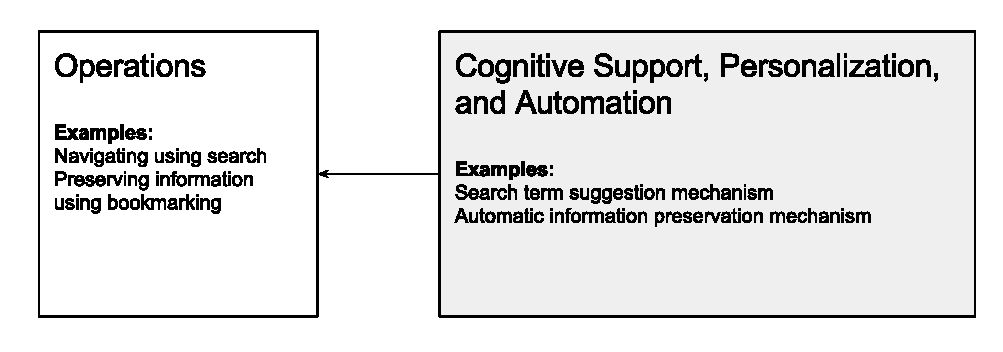
\includegraphics[width=\linewidth]{enhancement.pdf}
	\caption{Section Overview: Enhancing Information Discovery and Curation Experience}
	\label{fig:enhancement} 
\end{figure}
The information discovery and curation enablers presented in the previous section are design elements that afford various operations. For example, the search feature enables typing in a query and searching for information. These operations can be further aided by another set of design elements that introduce cognitive support, personalization, and automation. A high-level overview of this part of the framework is illustrated in Figure~\ref{fig:enhancement}. The primary goal of this part is to highlight opportunities for improvement over various information discovery and curation enabling mechanisms.

Strategies for improvement include providing additional cognitive support for a given operation, personalizing the user experience, and automating an operation. Not all of the strategies are feasible for every single operation, and some operations can be supported in multiple ways. The following sections outline some of the possibilities for advancing information discovery and curation features. 

{\subsection{Enhancing Navigation}
There are two common methods of enhancing information discovery when search-based navigation is used (see Table~\ref{table:navigation_support}). The first method entails returning personalized results when the user enters a search query. \textbf{Personalization} can be accomplished using a variety of techniques, including predefined user preferences, social interactions, context, browsing history, etc. The second method is to \textbf{suggest search terms} to make it easier for the user to formulate their information need. For example, Yelp suggests search terms as the user enters their query.

To further support referential navigation, applications can \textbf{personalize} reference suggestions, such as \textbf{categories}, \textbf{tags}, and \textbf{topics} of interest. They can also suggest relevant resources based on the one that the user already selected. As an example, after a user clicks a `pin', Pinterest showcases other similar `pins'.

For opportunistic navigation, Web tools sometimes allow users to \textbf{personalize} types or categories of information that they the users would like to discover. StumbleUpon allows users to not only choose topics of interests, but it can also help them discover new promising topics.

\begin{table}[ht!]
\caption{Cognitive Support, Automation, and Personalization for Navigation}
\label{table:navigation_support}
\begin{tabular}{{| >{\raggedright}p{0.35\linewidth}|p{0.60\linewidth}|}}
\hline
Support, automation, and personalization elements & Questions to be posed during the design or evaluation of discovery and curation tools \\
\hline
& \\
\textbf{Descriptional}       & \\
Personalized results         & Does the search mechanism return personalized results? \\
Guided search                & Does the system suggest search terms to the user? \\
& \\
\textbf{Referential}         & \\
Suggesting categories & Does the system suggest categories of interest? \\
Suggesting topics of interest & Does the system suggest topics of interest? \\
Suggesting tags              & Does the system suggest similar tags? \\
Suggesting similar resources & Does the system suggest similar resources? \\
& \\
\textbf{Opportunistic} & \\
Personalized opportunistic navigation     & Is it possible to personalize opportunistic navigation? \\
& \\
\textbf{System-regulated} & \\
Personalized featured content         & Is featured content personalized to the user? \\                                                       
User activity update notification & Is it possible to receive notifications about other users' activities? \\
Application activity update notification & Is it possible to receive notifications about website content updates?\\
Artifact update notification & Is it possible to receive notifications about artifact-related updates? \\                                                       
\hline

\end{tabular}
\end{table}
\clearpage

Featured content can also be \textbf{personalized} to improve information discovery with system-regulated navigation. For example, Yelp showcases restaurants from a predefined area, such as the city where the user is from.

Finally, to make better use of subscribed content and reduce human efforts when searching for information, an application can support various \textbf{notification mechanisms}. These mechanisms can advise the user about updates on the \textbf{Website content}, various \textbf{artifacts}, and activities of other \textbf{users}.  

} % end subsection
{\subsection{Enhancing Exploration}
\textbf{Personalization} of the \textbf{spatial} information representation usually has limited support in Web applications. Presumably, it is because consistency is more welcomed within information discovery applications than spatial personalization. However, it is still possible to personalize the arrangement of multiple resources or information within a single resource (see Table~\ref{table:exploration_support}). 

\textbf{Visual} and \textbf{textual personalizations} are more common, especially when the content within the application is curated by its users.  For example, Flickr Web application for managing and sharing photographs personalizes album covers so that they are easier to rediscover. Similarly, `pinboards' on Pinterest have personalized cover images.

\begin{table}[ht!]
\caption{Visual and Spatial Exploration Cognitive Support and Personalization}
\label{table:exploration_support}
\begin{tabular}{{| >{\raggedright}p{0.33\linewidth}|p{0.62\linewidth}|}}
\hline
Cognitive support and personalization design elements & Questions to be posed during the design or evaluation of discovery and curation tools  \\
\hline
 &\\
\textbf{Visual and textual cues of multiple resources} & \\
&\\
Personalized visual preview  & Does the system personalize visual previews of resources? \\
Personalized textual preview & Does the system personalize textual previews of resources? \\
& \\
\textbf{Visual and textual cues of a single resource} & \\
Personalized visual cues                 & Does the system personalize the visual cues within a resource? \\
Personalized textual cues                & Does the system personalize the textual cues within a resource? \\
\textbf{Spatial proximal cues of multiple resources} & \\
Personalized arrangement of multiple resources & Does the system personalize the arrangement of resources? \\  
& \\                                                  
\textbf{Spatial proximal cues of a single resource} & \\
Personalized arrangement of information within a resource          & Does the system personalize the arrangement of information within a resource? \\                                                       
& \\
\hline
\end{tabular}
\end{table}
} % end subsection

{\subsection{Enhancing Curation}

\begin{table}[ht!]
\caption{Cognitive Support, Personalization, and Automation for Curation}
\label{table:curation_support}
\begin{tabular}{{| >{\raggedright}p{0.30\linewidth}|p{0.65\linewidth}|}}
\hline
Cognitive support, personalization, and automation elements & Questions to be posed during the design or evaluation of information discovery and curation tools \\
\hline
& \\
\textbf{Management}		& \\
Suggesting collections  & Does the system suggest relevant collections? \\
Suggesting tags         & Does the system suggest relevant tags? \\
Automated classification into collections  	& Does the system automatically sort resources into collections? \\
Automated tagging       & Does the system automatically tag resources? \\
& \\
\textbf{Preservation}   & \\
History       			& Does the system automatically preserve information found by the user? \\
Suggested preservation  & Does the system suggest preservation channels to the user? \\
\textbf{Augmentation} 	& \\
Automated augmentation  & Does the system automatically annotate resources? \\
Suggested augmentation  & Does the system suggest annotation options to the user? \\    
& \\
\textbf{Sharing}        & \\
Automated sharing		& Does the system support automatic sharing? \\
Suggested sharing		& Does the system suggest sharing channels to the user? \\
& \\
\textbf{Subscription}   & \\
Suggesting users for subscription & Does the system suggest which users to subscribe to? \\
Suggesting artifacts for subscription   & Does the system suggest which artifacts to subscribe to? \\ 
Automated subscription  & Can the system automatically subscribe the user to the website activity? \\
&\\
\hline  
\end{tabular}
\end{table}

Information management can be improved if the system helps the user make decisions about information categorization or tagging (see Table~\ref{table:curation_support}). Alternatively, information can be \textbf{categorized} or \textbf{tagged automatically}. For example, when the user bookmarks a restaurant on Yelp, it is automatically categorized. The user can filter bookmarks by category whenever they go into the embedded bookmark manager. 

Preservation operations can also be automated. An example of the most common automatic preservation mechanism is \textbf{history}. Applications such as YouTube and Google Maps preserve users' browsing history so that they can review it later. Additionally, preservation mechanisms can be \textbf{suggested} to the user.

\pagebreak

YouTube allows users to \textbf{automatically share} information about their activities, such as comments,  added videos, liked or disliked videos, and created playlists. In general, socially curated spaces \textbf{offer sharing channels} to support convenient information communication.
 
Augmentation is another aspect of information curation that can be either \textbf{automated} for or \textbf{suggested} to the user. For example, Yelp asks users to rate the places which the application identifies as having been visited by the user. 

\pagebreak

Notification mechanisms enable user awareness about new content on the subscribed channel~\cite{millen2005social}. Web applications that facilitate rapidly updating content support various notification mechanisms, such as messages within the application, informative emails, and smartphone notifications. Many types of notifications include suggested users or artifacts to follow. Some Web tools automatically subscribe users to notifications, usually during the registration process.
} % end subsection
{\subsection{Summary}
Providing cognitive support, personalization, and automation dramatically improves the user experience when people interact with information discovery and curation systems. The framework can be used for identifying gaps in information discovery support and developing new technologies (see Chapters~\ref{chapter:application} and~\ref{chapter:evaluation}).  
}
}







